%%%%%%%%%%%%%%%%%%%%%%%%%%%%%%%%%%%%%%%%%
% Thin Sectioned Essay
% LaTeX Template
% Version 1.0 (3/8/13)
%
% This template has been downloaded from:
% http://www.LaTeXTemplates.com
%
% Original Author:
% Nicolas Diaz (nsdiaz@uc.cl) with extensive modifications by:
% Vel (vel@latextemplates.com)
%
% License:
% CC BY-NC-SA 3.0 (http://creativecommons.org/licenses/by-nc-sa/3.0/)
%
%%%%%%%%%%%%%%%%%%%%%%%%%%%%%%%%%%%%%%%%%

%----------------------------------------------------------------------------------------
%	PACKAGES AND OTHER DOCUMENT CONFIGURATIONS
%----------------------------------------------------------------------------------------

\documentclass[a4paper, 11pt]{article} % Font size (can be 10pt, 11pt or 12pt) and paper size (remove a4paper for US letter paper)

\usepackage{amssymb}
\usepackage{amsmath}
\usepackage{indentfirst}
\usepackage{amsthm}
\usepackage{cite}
\usepackage{bbding}
\usepackage{array}
\usepackage{graphicx}
\usepackage{epstopdf}
\usepackage[lined,boxed,commentsnumbered,ruled]{algorithm2e}
\usepackage[colorlinks,urlcolor=blue]{hyperref}
\usepackage[all,cmtip]{xy}
\usepackage{multicol}
\usepackage{color}
\usepackage{subfigure}

\usepackage[protrusion=true,expansion=true]{microtype} % Better typography
\usepackage{graphicx} % Required for including pictures
\usepackage{wrapfig} % Allows in-line images
\usepackage{booktabs}

\usepackage{mathpazo} % Use the Palatino font
\usepackage[T1]{fontenc} % Required for accented characters
\linespread{1.05} % Change line spacing here, Palatino benefits from a slight increase by default

\makeatletter
\renewcommand\@biblabel[1]{\textbf{#1.}} % Change the square brackets for each bibliography item from '[1]' to '1.'
\renewcommand{\@listI}{\itemsep=0pt} % Reduce the space between items in the itemize and enumerate environments and the bibliography

\renewcommand{\maketitle}{ % Customize the title - do not edit title and author name here, see the TITLE block below
\begin{flushright} % Right align
{\LARGE\@title} % Increase the font size of the title

\vspace{50pt} % Some vertical space between the title and author name

{\large\@author} % Author name
\\\@date % Date

\vspace{40pt} % Some vertical space between the author block and abstract
\end{flushright}
}

%----------------------------------------------------------------------------------------
%	TITLE
%----------------------------------------------------------------------------------------

\title{\textbf{A Predictor of DOTA2}\\ % Title
Machine Learning Project Report} % Subtitle

\author{\textsc{Wang Xiaohui, Yang Guang, Yang Yi, Zhuo Yiwei} % Author
\\{\textit{1140339072}}} % Institution

\date{\today} % Date

%----------------------------------------------------------------------------------------

\begin{document}

\maketitle % Print the title section

%----------------------------------------------------------------------------------------
%	ABSTRACT AND KEYWORDS
%----------------------------------------------------------------------------------------

%\renewcommand{\abstractname}{Summary} % Uncomment to change the name of the abstract to something else

\begin{abstract}
In this work, we collected the practical match data of DOTA2, and based on the data, we introduced two research on predicting the match result based on Support Vector Machine (SVM) and Convolutional Neural Networks (CNN). In order to find which parameter determines the result of the match, we exploit SVM to analyze all 11 parameters and find their weights in deciding the match result. And we find out several key parameters that players should focus on since these parameters have an outstanding influence on winning the game. In order to give an advice for players whether should they give up the ongoing game based on historical match data, we exploit CNN to make a prediction based on all 11 data items. We reached a 98.33\% prediction accuracy based on our trained CNN classifier model. 
\end{abstract}

\hspace*{3,6mm}\textit{Keywords:} SVM , CNN , Predictor, DOTA2 % Keywords

\vspace{30pt} % Some vertical space between the abstract and first section

%----------------------------------------------------------------------------------------
%	ESSAY BODY
%----------------------------------------------------------------------------------------

\section{Background and Motivation}
Each match of Dota 2 is independent and involves two teams, the Radiant and the Dire, both containing five players and each occupying a stronghold at either end of the map. Located in each stronghold is a building called the "Ancient"; to win, a team must destroy the enemy's Ancient. Each player controls a "Hero" character and focuses on leveling up, collecting gold, acquiring items and fighting against the other team to achieve victory.

There are nine game modes and around 100 "Heroes" in Dota 2. Heroes are strategically powerful player-controlled units with unique special abilities; though many heroes fill similar roles as others, each confers different benefits and limitations to a team. These Heroes start off very weak early in the game, but level up their abilities and statistics as they accumulate experience, up to a maximum level of twenty-five. The Heroes' methods of combat are heavily influenced by their primary property, which can be Strength, Agility, or Intelligence. Most game modes provide teams with some preparation time before the game begins so that they can balance their hero selections, as the composition of the team can significantly affect their performance throughout the match. Because Dota 2 is highly team-oriented, the players must coordinate and plan with each other in order to achieve victory.\cite{dota2}

We start our work in order to give reliable advice for players to concentrate on certain indexes. Also, for many circumstances, although continuing the game and struggling for victory would be an active attitude, however we find that for most cases these strives rest in vain and this process would make great harm to players' sentiment. So we researched on the actual match data and wanted to derive a high-performance predictor to make a reliable recommendation for players on whether they should give up the remaining game.

\section{Retrieve Data}
We collected 100K randomly chosen pieces of actual match data for our research, and choose 90K data as our training set and 10K as the testing set. Each piece of dataset is a log of one match, and listed ten players who attends the match with 11 items for each player describing certain match parameter listed in Table 1.
\begin{table}[htbp]	
	\centering 
	\begin{tabular}{lcl}
		\toprule
		denies & the number of times a player denied a creep\\
		xp\_per\_min &  the player's total xp/min\\
		player\_slot & 8-bit, top bit true is team dire and last 2 bits means player slot\\
		kills & the number of kills the player got\\
		level & the player's final level\\
		deaths & the number of times the player died\\
		hero\_damage &  the amount of damage the player dealt to heroes\\
		last\_hits & the number of times a player last-hit a creep\\
		hero\_id & the numeric ID of the hero that the player used\\
		tower\_damage & the amount of damage the player dealt to towers\\
		gold\_per\_min & the player's total gold/min\\
		
		\bottomrule
	\end{tabular}
	\caption{\label{tab:test}11 Data items for each player in the dataset}
\end{table}

Figure 1 shows an sample of dataset from one match. We consider only the ten players' data items. All 100K matches are stored in plain text. We build a 3-Dimensional matrix of $10 \times 11 \times 100000$, storing all data items in the sequence of Table 1 above as our input. And we build a vector of 100000 elements tagged the labels of the inputs in the same sequence.
\begin{figure}[h]
	\centering 
	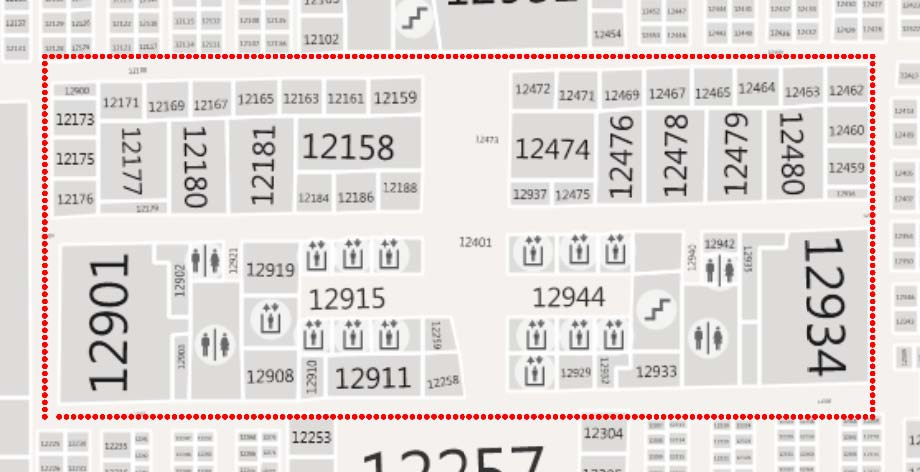
\includegraphics[width=1.0\linewidth]{Figure1.png}
	\caption{An example of one data sample of a match}
	\label{fig:subfig}
\end{figure}

\section{Exploit SVMs to verify the decisive factors}

\subsection{Necessity to verify individually}
We are all the youth who have played or have heard some video games. As to the issue of finding out a good enough prediction of Dota2, our experiences and intuitions naturally tell us: There are many factors that may affect the result differently, such as the hero familiarity of its controller, the skill of this match, the mistake or accident during the match. 
From the data set, actually we found there are 11 items for each player in a match, which are identified as $denies$, $xp\_per\_min$, $player\_slot$, $kills$, $level$, $deaths$, $hero\_damage$, $last\_hits$, $hero\_id$, $tower\_damage$ and $gold\_per\_min$ respectively. They are all the information we can make use of. We are asked by the proposer to use the items of "hero-id" and "level" only to predict the winner originally. But our group doubt whether or not the hero composition and the level of players truly are the most decisive factors. If the answer is negative, the accuracy of some machine learning method can be poor and meaningless. So one of our key points is that we need to figure out how much the single item associate with the accuracy of prediction result individually.


\subsection{Apply SVMs efficiently}
Our data set, with the size of 100,000 matches, can be regarded as a 10*11*10,000 three-dimensional matrix. It's a mid-size data! Fortunately, through the course of Machine Learning, we know: 1) SVMs, which are among the best (and many believe is indeed the best) "off-the-shelf" supervised learning algorithm; 2) Kernel trick, which give a way to apply SVMs efficiently in very high dimensional feature spaces. So we choose to use the algorithm of kernel trick which should be suitable to solve this problem.
Since the story of SVMs has been told in detail in our class, here we just simply summarize our idea as follows: 
Firstly, we divide 100,000 pieces of match data into two parts, 90,000 pieces for training, 10,000 pieces for testing. 
Secondly, execute like following pseudo-code.\\
1.	iterator  i = 1 : 11  \\
2.	SvmTrainData(i, 1:90000)\\
3.	SvmTestData(i,90001:100000)\\

\subsection{Reveal the truly most decisive factors}

We make a bar graph to conclude the accuracy of prediction results using 11 kinds 
of items individually as follows.
\begin{figure}[h]
	\centering 
	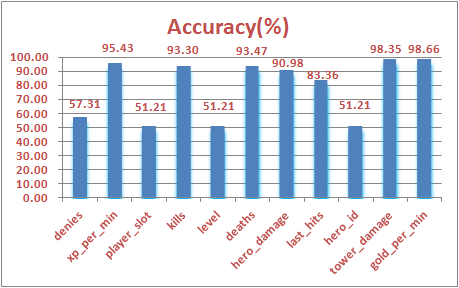
\includegraphics[width=0.8\linewidth]{Figure3.png}
	\caption{CNN Reduces Parameters}
	\label{fig:subfig}
\end{figure}

As we can see, two most decisive factors are "gold\_per\_min" and "tower\_damage" rather than "hero\_damage" and "level".We further infer the accuracy of prediction results may be just so so if we only use the items of "hero-id" and "level".What we discover is coincident with the baseline, given by the proposer, which gets 61\% of accuracy. It seems to draw a conclusion the more money you earn and the more damage you bring to your enemy's tower, the higher probability you will win.


\section{Exploiting CNN to make a prediction on whether should we give up}
\subsection{Convolutional Neural Networks}
Convolutional Neural Networks is a type of feed-forward artificial neural network where the individual neurons are tiled in such a way that they respond to overlapping regions in the visual field.\cite{CNN1} A CNN is comprised of one or more convolutional layers (often with a subsampling step) and then followed by one or more fully connected layers as in a standard multilayer neural network.\cite{CNN2} For each layer of the network, 
The benefits of CNN is that it can dramatically reduce the amount of parameters that should be trained. As the figure shows below, if we obtain $1000 \times 1000$ pixels, with 1M hidden neurons, and for each neuron it should connect each pixel of the image, then there exists $10^{12}$ connections, which needs to train $10^{12}$ parameters. However, the spatial connection of the image is localized, so one neuron doesn't have to comprehend the total details of the image, and only need to read the local part of the image. And in upper layer we can synthesis different parts so that we get the global information. By this we can dramatically reduce the amount of connections. Suppose one nueron need only to connect with $10 \times 10$ pixels, the total amount of connection is $10^8$.
\begin{figure}[h]
	\centering 
	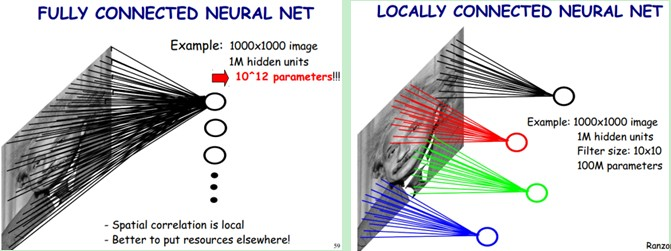
\includegraphics[width=0.8\linewidth]{Figure2.jpg}
	\caption{CNN Reduces Parameters}
	\label{fig:subfig}
\end{figure}

In fact, we can apply same parameters for every neuron, so the parameters we need to train draws down to $10 \times 10$.

\subsection{Network Design}


\subsection{Train the Network}
Before we set the structured data discussed in section 2, we need to initialize the data by using each match data items subtract the average value of all matches.

We need to train a classifier with an output label with "insist on" or "give up". The training set consists of m labeled samples \{${(x^{(1)},y^{(1)}),(x^{(2)},y^{(2)}), \dots,(x^{(m)},y^{(m)})}$\}, and the input feature vector $x^{(i)} \in \mathbb{R^{N+1}}$ with $x_0 = 1$ corresponding to the interception item and $\mathbb{N}$ here refer to 11. We exploit softmax regression for this binary-classifier. Because label $y^{(i)} \in \{0,1\}$, so in this condition Softmax degenerated into logistic regression. The hypothesis function listed as below:
 \begin{equation*}
 \centering
 h_\theta(x) = \frac{1}{1+exp(-\theta^Tx)}
 \end{equation*}
We will train the parameter $\theta$ in order to minimize the cost function below, and we adopted gradient descent to minimize $J(\theta)$.
 \begin{equation*}
 \centering
 J(\theta) = -\frac{1}{m}[\sum_{i=1}^{m}y^{(i)}logh_\theta(x^{(i)})+(1-y^{(i)})log(1-h_\theta(x^{(i)}))]
 \end{equation*}
 

\subsection{Prediction Evaluation}
We performed the experiment using Matlab, and reached an accuracy of 98.33\% prediction accuracy rate.
Figure 4(a) shows the change of loss function $J(\theta)$ during the training process. Figure 4(b) shows the error prediction rate of the testing set. We perform the testing process once after the network updates its parameters by randomly choose 500 matches from the testing set.
\begin{figure}[h]
	\centering 
	\subfigure[loss function]{ 
		\label{fig:subfig:a} 
		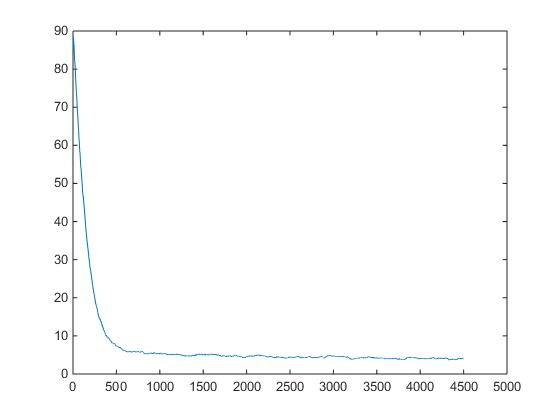
\includegraphics[width=0.4\linewidth]{cnn_lossfunction.jpg}} 
	\subfigure[test error rate]{
		\label{fig:subfig:b} 
		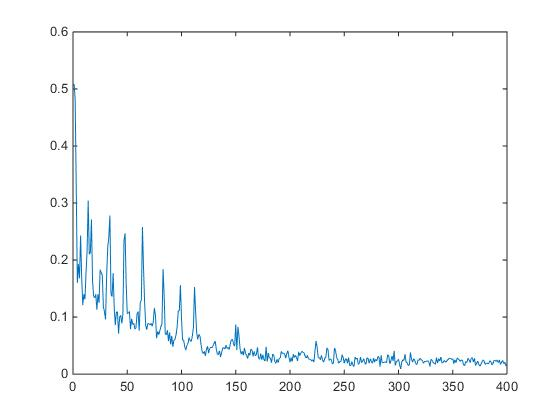
\includegraphics[width=0.4\linewidth]{cnn_test_error_rate.jpg}}
	\caption{The results of CNN}
	\label{fig:subfig}
\end{figure}

\section{Evaluation and Conclusion}
We draw the conclusion that one should focus on earning money and bring damage to towers of the foes so that they would be more possible to win a match. We exploits SVM to implement this feature.
We also trained a reliable model that can provide reliable recommendation of whether you should give up or insist on based on the retrieved data of the ongoing match. We exploits CNN to implement this feature.

%----------------------------------------------------------------------------------------
%	BIBLIOGRAPHY
%----------------------------------------------------------------------------------------

\begin{thebibliography}{10}

\bibitem[1]{Radar00}
P.Bahl, V.N. Padmanabhan,
``Radar: An in-building RF-Based User Location and Tracking System.''
\textit{Proc. of IEEE INFOCOM}, volumn 2, pp. 775-784, 2000.

\bibitem[2]{dota2}
``$www.en.wikipedia.org/wiki/Dota\_2$''
\textit{WikiPedia}

\bibitem[3]{CNN1}
``$www.en.wikipedia.org/wiki/Convolutional\_neural\_network$''
\textit{WikiPedia}

\bibitem[4]{CNN2}
``$www.ufldl.stanford.edu/tutorial/supervised/ConvolutionalNeuralNetwork/$''
\textit{Stanford}
\end{thebibliography}

%----------------------------------------------------------------------------------------

\end{document}